%
% Vienna University of Technology - Faculty of Informatics
% TUINF thesis - LaTeX template
%
% For questions and comments send an email to
% Thomas Auzinger <thomas.auzinger@cg.tuwien.ac.at>
% Thomas Krennwallner <tkren@kr.tuwien.ac.at>
%
% ---------------------------------------------------------
%
% TU Wien - Fakultät für Informatik
% TUINF Arbeit - Template für LaTeX
%
% Für Fragen oder Kommentare schicken Sie eine Email an
% Thomas Auzinger <thomas.auzinger@cg.tuwien.ac.at>
% Thomas Krennwallner <tkren@kr.tuwien.ac.at>
%

\documentclass[a4paper,11pt]{memoir}
\chapterstyle{veelo}

\usepackage{TUINFTHESIS}

\usepackage{geometry}[2010/02/15] % page geometry (\newgeometry command needs a recent version)
\usepackage{url}      % URL functionality
\usepackage{hyperref} % hyperlinks in PDF files
\usepackage{graphicx} % images
\usepackage{verbatim} % code environments
\usepackage[lined,linesnumbered,algochapter]{algorithm2e} % algorithm environments

\usepackage{pgf}  % graphics
\usepackage{tikz}	% graphics
\usetikzlibrary{arrows,automata}

\usepackage{ngerman}           % support for German
\usepackage[ngerman]{babel}    % support for German
\usepackage{bibgerm,cite}      % German notations
\usepackage[ngerman]{varioref} % German references
% to use the german charset include cp850 for MS-DOS, ansinew for Windows and latin1 for Linux.
% \usepackage[latin1]{inputenc}

% enable hyphenation of urls at every location (to avoid bad boxes)
\renewcommand{\UrlBreaks}{\do\/\do\a\do\b\do\c\do\d\do\e\do\f\do\g\do\h\do\i\do\j\do\k\do\l\do\m\do\n\do\o\do\p\do\q\do\r\do\s\do\t\do\u\do\v\do\w\do\x\do\y\do\z\do\A\do\B\do\C\do\D\do\E\do\F\do\G\do\H\do\I\do\J\do\K\do\L\do\M\do\N\do\O\do\P\do\Q\do\R\do\S\do\T\do\U\do\V\do\W\do\X\do\Y\do\Z}

% all the following \thesis... definitions are mandatory unless declared optional
\thesistitle{Titel}
\thesissubtitle{Optional Subtitle} % optional
\thesisdate{TT.MM.JJJJ}
\thesislocation{Wien}

\thesistype{master} % master or bachelor
\thesiscurriculum{Medieninformatik und Visual Computing}{Media Informatics and Visual Computing} % German and English

\thesisauthorname{Martina Muster}
\thesisauthorgender{female} % female or male
\thesisauthoraddress{Musterplatz 1, 1111 Wien}
\thesismatrikelno{0123456}

\thesisadvisorname{o.Univ.-Prof. Dipl.-Ing. Mag. Dr. Monika Musterprofessorin}
\thesisadvisorgender{female} % female or male
\thesisassistantonename{Dr. Vorname Familienname}
\thesisassistanttwoname{Dr. Vorname Familienname} % optional

\begin{document}

\captionnamefont{\bfseries}

% define page numbering styles
\makepagestyle{numberCorner}
\makeevenfoot{numberCorner}{\thepage}{}{}
\makeoddfoot{numberCorner}{}{}{\thepage}

%%%%%%%%%%%%%%%%%%%%%%%%%%%%%%%%%%%%%%%%%
%%%   FRONTMATTER    %%%%%%%%%%%%%%%%%%%%
%%%%%%%%%%%%%%%%%%%%%%%%%%%%%%%%%%%%%%%%%
\frontmatter
\pagenumbering{roman}

%%%%%%%%%%%%%%%%%%%%%%%%%%%%%%%%%%%%%%%%%
%%%   TITLE PAGES    %%%%%%%%%%%%%%%%%%%%
%%%%%%%%%%%%%%%%%%%%%%%%%%%%%%%%%%%%%%%%%
%
% Vienna University of Technology - Faculty of Informatics
% TUINF thesis - Title page German
%
% For questions and comments send an email to
% Thomas Auzinger <thomas.auzinger@cg.tuwien.ac.at>
% Thomas Krennwallner <tkren@kr.tuwien.ac.at>
%
% ---------------------------------------------------------
%
% TU Wien - Fakult�t f�r Informatik
% TUINF Arbeit - Titelseite deutsch
%
% F�r Fragen oder Kommentare schicken Sie eine Email an
% Thomas Auzinger <thomas.auzinger@cg.tuwien.ac.at>
% Thomas Krennwallner <tkren@kr.tuwien.ac.at>
%

\selectlanguage{ngerman}

% setup page dimensions for the titlepage
\newgeometry{left=2.4cm,right=2.4cm,bottom=2.5cm,top=2cm}

% force baselineskip and parindent
\newlength{\tmpbaselineskip}
\setlength{\tmpbaselineskip}{\baselineskip}
\setlength{\baselineskip}{13.6pt}
\newlength{\tmpparindent}
\setlength{\tmpparindent}{\parindent}
\setlength{\parindent}{17pt}

% title page
\thispagestyle{tuinftitlepage}

% Prevent warning messages due to tall headers
\addtolength{\headheight}{65pt}
\addtolength{\headsep}{-65pt}

%
% Kludge: for each titlepage set \pagenumbering to a different
% style. This is used to fix a problem with hyperref, because there
% are multiple "page 1" and hyperref hates that
%
\pagenumbering{Roman}

\begin{center}
{\ \vspace{3.4cm}}

\begin{minipage}[t][2.8cm][s]{\textwidth}%
\centering
\thesistitlefontHUGE\sffamily\bfseries\tuinfthesistitle\\
\bigskip
{\thesistitlefonthuge\sffamily\bfseries\tuinfthesissubtitle}
\end{minipage}

\vspace{1.3cm}

{\thesistitlefontLARGE\sffamily \tuinfthesistypename}

\vspace{6mm}

{\thesistitlefontlarge\sffamily zur Erlangung des akademischen Grades}

\vspace{6mm}

{\thesistitlefontLARGE\sffamily\bfseries \tuinfthesisdegree}

\vspace{6mm}

{\thesistitlefontlarge\sffamily im Rahmen des Studiums}

\vspace{6mm}

{\thesistitlefontLarge\sffamily\bfseries \tuinfthesiscurriculum}

\vspace{6.5mm}

{\thesistitlefontlarge\sffamily eingereicht von}

\vspace{6mm}

{\thesistitlefontLarge\sffamily\bfseries \tuinfthesisauthorname}

\vspace{1.5mm}

{\thesistitlefontlarge\sffamily Matrikelnummer \tuinfthesismatrikelno} 

\vspace{1.4cm}

\begin{minipage}[t][1.6cm][t]{\textwidth}%
	\vspace{0pt}\raggedright\thesistitlefontnormalsize\sffamily%
  an der Fakult\"{a}t f\"{u}r Informatik
	
	der Technischen Universit\"{a}t Wien
\end{minipage}

\begin{minipage}[t][4cm][t]{\textwidth}%
  \vspace{0pt}\raggedright\thesistitlefontnormalsize\sffamily%
  \begin{tabbing}%
	    \hspace{19mm} \= \hspace{66mm} \kill
	    Betreuung: \> \tuinfthesisadvisorname\\
	    Mitwirkung: \> \tuinfthesisassistantonename\\
	                \> \tuinfthesisassistanttwoname
  \end{tabbing}
\end{minipage}

\begin{minipage}[t][1.5cm][t]{\textwidth}%
  \vspace{0pt}\sffamily\thesistitlefontnormalsize
  \begin{tabbing}%
    \hspace{45mm} \= \hspace{63mm} \= \hspace{51mm} \kill
    Wien, \tuinfthesisdate \> {\raggedright\rule{51mm}{0.5pt}} \> {\raggedright\rule{51mm}{0.5pt}} \\
    \> \begin{minipage}[t][0.5cm][t]{51mm}\centering (Unterschrift \tuinfthesisverfasser)\end{minipage}
    \> \begin{minipage}[t][0.5cm][t]{51mm}\centering (Unterschrift \tuinfthesisbetreuer)\end{minipage}
    \end{tabbing}
\end{minipage}

\end{center}

% we want an empty page right after first titlepage
\pagestyle{empty}
\cleardoublepage

% we're done with the titlepages, proceed with default pagenumbering
\pagenumbering{roman}

% restore baselineskip
\setlength{\baselineskip}{\tmpbaselineskip}
\setlength{\parindent}{\tmpparindent}

% back to normal geometry
\restoregeometry % the German title page is required as first page
%
% Vienna University of Technology - Faculty of Informatics
% TUINF thesis - Title page English
%
% For questions and comments send an email to
% Thomas Auzinger <thomas.auzinger@cg.tuwien.ac.at>
% Thomas Krennwallner <tkren@kr.tuwien.ac.at>
%
% ---------------------------------------------------------
%
% TU Wien - Fakult�t f�r Informatik
% TUINF Arbeit - Titelseite englisch
%
% F�r Fragen oder Kommentare schicken Sie eine Email an
% Thomas Auzinger <thomas.auzinger@cg.tuwien.ac.at>
% Thomas Krennwallner <tkren@kr.tuwien.ac.at>
%

\selectlanguage{english}

% setup page dimensions for the titlepage
\newgeometry{left=2.4cm,right=2.4cm,bottom=2.5cm,top=2cm}

% force baselineskip and parindent
\newlength{\tmpbaselineskipen}
\setlength{\tmpbaselineskipen}{\baselineskip}
\setlength{\baselineskip}{13.6pt}
\newlength{\tmpparindenten}
\setlength{\tmpparindenten}{\parindent}
\setlength{\parindent}{17pt}

% title page
\thispagestyle{tuinftitlepage}

% Prevent warning messages due to tall headers
\addtolength{\headheight}{65pt}
\addtolength{\headsep}{-65pt}

%
% Kludge: for each titlepage set \pagenumbering to a different
% style. This is used to fix a problem with hyperref, because there
% are multiple "page 1" and hyperref hates that
%
\pagenumbering{Alph}

\begin{center}
{\ \vspace{3.4cm}}

\begin{minipage}[t][2.8cm][s]{\textwidth}%
\centering
\thesistitlefontHUGE\sffamily\bfseries\tuinfthesistitle\\
\bigskip
{\thesistitlefonthuge\sffamily\bfseries\tuinfthesissubtitle}
\end{minipage}

\vspace{1.3cm}

{\thesistitlefontLARGE\sffamily \tuinfthesistypenameen}

\vspace{6mm}

{\thesistitlefontlarge\sffamily submitted in partial fulfillment of the requirements for the degree of}

\vspace{6mm}

{\thesistitlefontLARGE\sffamily\bfseries \tuinfthesisdegree}

\vspace{6mm}

{\thesistitlefontlarge\sffamily in}

\vspace{6mm}

{\thesistitlefontLarge\sffamily\bfseries \tuinfthesiscurriculumen}

\vspace{6.5mm}

{\thesistitlefontlarge\sffamily by}

\vspace{6mm}

{\thesistitlefontLarge\sffamily\bfseries \tuinfthesisauthorname}

\vspace{1.5mm}

{\thesistitlefontlarge\sffamily Registration Number \tuinfthesismatrikelno} 

\vspace{1.4cm}

\begin{minipage}[t][1.6cm][t]{\textwidth}%
  \vspace{0pt}\raggedright\thesistitlefontnormalsize\sffamily%
  to the Faculty of Informatics 

  at the Vienna University of Technology
\end{minipage}

\begin{minipage}[t][4cm][t]{\textwidth}%
	\vspace{0pt}\raggedright\thesistitlefontnormalsize\sffamily
  \begin{tabbing}%
	    \hspace{19mm} \= \hspace{66mm} \kill
	    Advisor: \> \tuinfthesisadvisorname\\
	    Assistance: \> \tuinfthesisassistantonename\\
	                \> \tuinfthesisassistanttwoname
   \end{tabbing}
\end{minipage}

\begin{minipage}[t][1.5cm][t]{\textwidth}%
  \vspace{0pt}\sffamily\thesistitlefontnormalsize
  \begin{tabbing}%
    \hspace{45mm} \= \hspace{63mm} \= \hspace{51mm} \kill
    Vienna, \tuinfthesisdate \> {\raggedright\rule{51mm}{0.5pt}} \> {\raggedright\rule{51mm}{0.5pt}} \\
    \> \begin{minipage}[t][0.5cm][t]{51mm}\centering (Signature of Author)\end{minipage}
    \> \begin{minipage}[t][0.5cm][t]{51mm}\centering (Signature of Advisor)\end{minipage}
    \end{tabbing}
\end{minipage}

\end{center}

% we want an empty page right after first titlepage
\pagestyle{empty}
\cleardoublepage

% we're done with the titlepages, proceed with default pagenumbering
\pagenumbering{roman}

% restore baselineskip
\setlength{\baselineskip}{\tmpbaselineskipen}
\setlength{\parindent}{\tmpparindenten}

% back to normal geometry
\restoregeometry % optional English title page

%%%%%%%%%%%%%%%%%%%%%%%%%%%%%%%%%%%%%%%%%
%%%   DECLARATION OF ORIGINALITY    %%%%%
%%%%%%%%%%%%%%%%%%%%%%%%%%%%%%%%%%%%%%%%%
\cleardoublepage
%
% Vienna University of Technology - Faculty of Informatics
% TUINF thesis - Declaration of originality
%
% For questions and comments send an email to
% Thomas Auzinger <thomas.auzinger@cg.tuwien.ac.at>
% Thomas Krennwallner <tkren@kr.tuwien.ac.at>
%
% ---------------------------------------------------------
%
% TU Wien - Fakultät für Informatik
% TUINF Arbeit - Verfassungserklärung
%
% Für Fragen oder Kommentare schicken Sie eine Email an
% Thomas Auzinger <thomas.auzinger@cg.tuwien.ac.at>
% Thomas Krennwallner <tkren@kr.tuwien.ac.at>
%

\selectlanguage{ngerman}

\chapter*{Erklärung zur Verfassung der Arbeit}

\tuinfthesisauthorname\\
\tuinfthesisauthoraddress

\vspace*{1.2cm}
Hiermit erkläre ich, dass ich diese Arbeit selbständig verfasst habe, dass ich die verwendeten Quellen und Hilfsmittel vollständig angegeben habe und dass ich die Stellen der Arbeit -- einschließlich Tabellen, Karten und Abbildungen --, die anderen Werken oder dem Internet im Wortlaut oder dem Sinn nach entnommen sind, auf jeden Fall unter Angabe der Quelle als Entlehnung kenntlich gemacht habe.\\
\vspace*{2cm}
\begin{tabbing}%
    \hspace{58mm} \= \hspace{28mm} \= \hspace{58mm} \kill
    {\raggedright\rule{58mm}{0.5pt}} \> \> {\raggedright\rule{58mm}{0.5pt}} \\
    \begin{minipage}[t][0.5cm][t]{58mm}
	\vspace{0pt}\sffamily\thesistitlefontnormalsize
	\centering (Ort, Datum)
    \end{minipage}
    \> \>
    \begin{minipage}[t][0.5cm][t]{58mm}
	\vspace{0pt}\sffamily\thesistitlefontnormalsize
	\centering (Unterschrift \tuinfthesisverfasser)
    \end{minipage}
\end{tabbing} % the declaration of originality is mandatory

%%%%%%%%%%%%%%%%%%%%%%%%%%%%%%%%%%%%%%%%%
%%%   ACKNOWLEDGEMENTS    %%%%%%%%%%%%%%%
%%%%%%%%%%%%%%%%%%%%%%%%%%%%%%%%%%%%%%%%%
%
% Vienna University of Technology - Faculty of Informatics
% TUINF thesis - Acknowledgements German
%
% For questions and comments send an email to
% Thomas Auzinger <thomas.auzinger@cg.tuwien.ac.at>
% Thomas Krennwallner <tkren@kr.tuwien.ac.at>
%
% ---------------------------------------------------------
%
% TU Wien - Fakultät für Informatik
% TUINF Arbeit - Danksagung deutsch
%
% Für Fragen oder Kommentare schicken Sie eine Email an
% Thomas Auzinger <thomas.auzinger@cg.tuwien.ac.at>
% Thomas Krennwallner <tkren@kr.tuwien.ac.at>
%

\selectlanguage{ngerman}

\chapter*{Danksagung}

Hier fügen Sie optional eine Danksagung ein.
 % optional
%
% Vienna University of Technology - Faculty of Informatics
% TUINF thesis - Acknowledgements English
%
% For questions and comments send an email to
% Thomas Auzinger <thomas.auzinger@cg.tuwien.ac.at>
% Thomas Krennwallner <tkren@kr.tuwien.ac.at>
%
% ---------------------------------------------------------
%
% TU Wien - Fakult�t f�r Informatik
% TUINF Arbeit - Danksagung englisch
%
% F�r Fragen oder Kommentare schicken Sie eine Email an
% Thomas Auzinger <thomas.auzinger@cg.tuwien.ac.at>
% Thomas Krennwallner <tkren@kr.tuwien.ac.at>
%

\selectlanguage{english}

\chapter*{Acknowledgements}

Optional acknowledgements may be inserted here. % optional

%%%%%%%%%%%%%%%%%%%%%%%%%%%%%%%%%%%%%%%%%
%%%   ABSTRACT    %%%%%%%%%%%%%%%%%%%%%%%
%%%%%%%%%%%%%%%%%%%%%%%%%%%%%%%%%%%%%%%%%
%
% Vienna University of Technology - Faculty of Informatics
% TUINF thesis - Abstract German
%
% For questions and comments send an email to
% Thomas Auzinger <thomas.auzinger@cg.tuwien.ac.at>
% Thomas Krennwallner <tkren@kr.tuwien.ac.at>
%
% ---------------------------------------------------------
%
% TU Wien - Fakultät für Informatik
% TUINF Arbeit - Kurzfassung deutsch
%
% Für Fragen oder Kommentare schicken Sie eine Email an
% Thomas Auzinger <thomas.auzinger@cg.tuwien.ac.at>
% Thomas Krennwallner <tkren@kr.tuwien.ac.at>
%

\selectlanguage{ngerman}

\chapter*{Kurzfassung}

Die Explosionsgrafik ist eine Technik der Illustrativen Visualisierung, die die Funktion oder den Aufbau eines komplexen Objekts darstellt, in dem es in seine Einzelteile zerlegt wird, die dann so im Raum platziert werden, dass sie im Idealfall vollständig sichtbar sind und sich durch ihre Position auf ihre ursprüngliche Position innerhalb des Objekts rückschließen lässt. Diese Bachelorarbeit beschäftigt sich mit der Implementierung eines Plug-Ins für die Visualisierungssoftware VolumeShop, das in der Lage ist aus zusammengesetzten Dreiecks-Meshes einfache Explosionsgrafiken dynamisch zu erzeugen. Da es sich hier um eine interaktive Visualierung handelt, bei der man vor Allem den Blickwinkel verändern kann, ist es möglich die grafik von einem Punkt nahe der ExplosionsAche zu betrachten. In diesem Fall würde die Explosionsdistanz sehr groß, wodurch die einzelnen Teile entweder sehr klein dargestellt oder ausserhalb des Bildes platziert würden. um dieses problem zu umgehen, wurde für diese Blickwinkel eine Kombination aus Explosionsgrafik und Ghosting eingesetzt. Ghosting ist eine andere Illustrationstechnik, bei der Objekte, die sich zwischen dem Betrachter und einem wichtigen Objekt befinden transparent dargestellt werden.
\cleardoublepage
%
% Vienna University of Technology - Faculty of Informatics
% TUINF thesis - Abstract English
%
% For questions and comments send an email to
% Thomas Auzinger <thomas.auzinger@cg.tuwien.ac.at>
% Thomas Krennwallner <tkren@kr.tuwien.ac.at>
%
% ---------------------------------------------------------
%
% TU Wien - Fakult�t f�r Informatik
% TUINF Arbeit - Kurzfassung englisch
%
% F�r Fragen oder Kommentare schicken Sie eine Email an
% Thomas Auzinger <thomas.auzinger@cg.tuwien.ac.at>
% Thomas Krennwallner <tkren@kr.tuwien.ac.at>
%

\selectlanguage{english}

\chapter*{Abstract}

Exploded view is a technique in illustrative visualization where the inner working of complex objects is revealed by segmenting it into several parts.They are then displaced so that ideally they are fully visible and their positions convey information about their original place in the object. This thesis deals with implementing a plug-in for the visualization software VolumeShop that is able to create simple dynamic exploding views from composite triangle meshes. Because the Illustration is interactive and can be viewed from all angles, the explosion distance becomes very large to infinite when looking at the object from a viewpoint close to the explosion axis.  To avoid this exploded views were combined with ghosting, which is a different illustrative technique where an object between the viewer and a more important object is drawn translucently.

%%%%%%%%%%%%%%%%%%%%%%%%%%%%%%%%%%%%%%%%%
%%%   SELECT LANGUAGE    %%%%%%%%%%%%%%%%
%%%%%%%%%%%%%%%%%%%%%%%%%%%%%%%%%%%%%%%%%
% results in "Inhaltsverzeichnis", "Kapitel", "Abbildung", or "Contents", "Chapter", and "Figure"
\selectlanguage{english}
%\selectlanguage{ngerman} % files that use umlaut characters (ä,ö,ü) need to be encoded in utf-8


%%%%%%%%%%%%%%%%%%%%%%%%%%%%%%%%%%%%%%%%%
%%%   CONTENTS    %%%%%%%%%%%%%%%%%%%%%%%
%%%%%%%%%%%%%%%%%%%%%%%%%%%%%%%%%%%%%%%%%
\setcounter{tocdepth}{1}
\cleardoublepage
\pagestyle{numberCorner}
\tableofcontents*

%%%%%%%%%%%%%%%%%%%%%%%%%%%%%%%%%%%%%%%%%
%%%   MAINMATTER    %%%%%%%%%%%%%%%%%%%%%
%%%%%%%%%%%%%%%%%%%%%%%%%%%%%%%%%%%%%%%%%
\mainmatter
\pagenumbering{arabic}
\pagestyle{numberCorner}

%%%%%%%%%%%%%%%%%%%%%%%%%%%%%%%%%%%%%%%%%
\chapter{Introduction}
\label{ch:intro}
%%%%%%%%%%%%%%%%%%%%%%%%%%%%%%%%%%%%%%%%%

\ifthenelse{\equal{\tuinfthesistype}{master}}
  {\section{General Information}

This document is intended as a template and guideline and should support the author in the course of doing the master's thesis.
Assessment criteria comprise the quality of the theoretical and/or practical work as well as structure, content and wording of the written master's thesis. Careful attention should be given to the basics of scientific work (e.g., correct citation).

\section{Organizational Issues}

A master's thesis at the Faculty of Informatics has to be finished within six months. During this period regular meetings between the advisor(s) and the author have to take place.
In addition, the following milestones have to be fulfilled:
\begin{enumerate}
  \item  Within one month after having fixed the topic of the thesis the master's thesis proposal has to be prepared and must be accepted by the advisor(s). The master's thesis proposal must follow the respective template of the dean of academic affairs. Thereafter the proposal has to be applied for at the deanery. The necessary forms may be found on the web site of the Faculty of Informatics. \url{http://www.informatik.tuwien.ac.at/dekanat/formulare.html}
  \item  Accompanied with the master's thesis proposal, the structure of the thesis in terms of a table of contents has to be provided.
  \item Then, the first talk has to be given at the so-called ``Seminar for Master Students''. The slides have to be discussed with the advisor(s) one week in advance. Attendance of the ``Seminar for Master Students'' is compulsory and offers the opportunity to discuss arising problems among other master students.
  \item At the latest five months after the beginning, a provisional final version of the thesis has to be handed over to the advisor(s).  
  \item As soon as the provisional final version exists, a first poster draft has to be made. The making of a poster is a compulsory part of the ``Seminar for Master Students'' for all master studies at the Faculty of Informatics. Drafts and design guidelines can be found at \url{http://www.informatik.tuwien.ac.at/studium/richtlinien}.
  \item After having consulted the advisor(s) the second talk has to be held at the ``Seminar for Master Students''.
  \item At the latest six months after the beginning, the corrected version of the master's thesis and the poster have to be handed over to the advisor(s).
  \item After completion the master's thesis has to be presented at the ``epilog''. For detailed information on the epilog see: \\ \url{http://www.informatik.tuwien.ac.at/studium/epilog}
\end{enumerate}

\section{Structure of the Master's Thesis}

If the curriculum regulates the language of the master's thesis to be English (like for ``Business Informatics''), the thesis has to be written in English. Otherwise, the master's thesis may be written in English or in German. The structure of the thesis is predetermined.
The table of contents is followed by the introduction and the main part, which can vary according to the content. The master's thesis ends with the bibliography (compulsory) and the appendix (optional).

\begin{itemize}
  \item	Cover page
  \item Acknowledgements
  \item Abstract of the thesis in English and German
  \item Table of contents
  \item Introduction
  	\begin{itemize}
  		\item motivation
  		\item problem statement (which problem should be solved?)
  		\item aim of the work
  		\item methodological approach
  		\item structure of the work
  	\end{itemize}
  \item State of the art / analysis of existing approaches
  	\begin{itemize}
  		\item literature studies
  		\item analysis
  		\item comparison and summary of existing approaches
  	\end{itemize}
  \item Methodology
  	\begin{itemize}
  		\item used concepts
  		\item methods and/or models
  		\item languages
  		\item design methods
  		\item data models
  		\item analysis methods
  		\item formalisms
  	\end{itemize}
  \item Suggested solution/implementation
  \item Critical reflection
  	\begin{itemize}
  		\item comparison with related work
  		\item discussion of open issues
  	\end{itemize}
  \item Summary and future work
  \item Appendix: source code, data models, \dots
  \item Bibliography
\end{itemize}

}
	{\section{General Information}

This document is intended as a template and guideline and should support the author in the course of doing the bachelor's thesis.
Assessment criteria comprise the quality of the theoretical and/or practical work as well as structure, content and wording of the written bachelor's thesis. Careful attention should be given to the basics of scientific work (e.g., correct citation).

\section{Structure of the Bachelor's Thesis}

If the curriculum regulates the language of the bachelor's thesis to be English, the thesis has to be written in English. Otherwise, the bachelor's thesis may be written in English or in German.
The table of contents is followed by the introduction and the main part, which can vary according to the content. The bachelor's thesis ends with the bibliography (compulsory) and the appendix (optional).

\begin{itemize}
  \item	Cover page
  \item Acknowledgments
  \item Abstract of the thesis in English and German
  \item Table of contents
  \item Introduction
  	\begin{itemize}
  		\item motivation
  		\item problem statement (which problem should be solved?)
  		\item aim of the work
  		\item methodological approach
  		\item structure of the work
  	\end{itemize}
  \item State of the art / analysis of existing approaches
  	\begin{itemize}
  		\item literature studies
  		\item analysis
  		\item comparison and summary of existing approaches
  	\end{itemize}
  \item Methodology
  	\begin{itemize}
  		\item used concepts
  		\item methods and/or models
  		\item languages
  		\item design methods
  		\item data models
  		\item analysis methods
  		\item formalisms
  	\end{itemize}
  \item Suggested solution/implementation
  \item Critical reflection
  	\begin{itemize}
  		\item comparison with related work
  		\item discussion of open issues
  	\end{itemize}
  \item Summary and future work
  \item Appendix: source code, data models, \dots
  \item Bibliography
\end{itemize}

}

%%%%%%%%%%%%%%%%%%%%%%%%%%%%%%%%%%%%%%%%%
\chapter{Typographic Design}
\label{ch:typo}
%%%%%%%%%%%%%%%%%%%%%%%%%%%%%%%%%%%%%%%%%

% define custom macros for specific formats or names
\newcommand{\uml}[1]{\texttt{#1}}
\newcommand{\cd}{\textsf{Class Diagram}}

For working with \LaTeX you can take advantage of a variety of books and free introductions and tutorials on the internet. A competent contact point for \LaTeX beginners is the \LaTeX Wikibook, which is available under \url{http://en.wikibooks.org/wiki/LaTeX}. 

The following sections give examples of the most important \LaTeX environments and commands.

\section{Tables}

Tables have to be realized with the help of the \textit{table} environment. Tables shall be sequentially numbered for each chapter and described in terms of a short caption (cf. Table~\ref{tab:diplomaseminar}).

\begin{table}[htb]
	\centering
	\begin{tabular}{|l|c|c|}
		\hline \textbf{Name} & \textbf{Date} & \textbf{Title} \\
		\hline
		\hline Mustermann Adam  & 18.5   & T1    \\
		\hline Musterfrau Eva  & 22.6   & T2    \\
		\hline
	\end{tabular}
	\caption{Seminar for Master Students}
	\label{tab:diplomaseminar}
\end{table}


\section{Figures}

Like tables, figures shall be sequentially numbered for each chapter and described in terms of a short caption). You could either produce your drawings directly inside \LaTeX using PSTricks\footnote{\url{http://tug.org/PSTricks}}, Tikz\footnote{\url{http://sourceforge.net/projects/pgf}}, or any set of macros dedicated to your requirements (cf. Figure~\ref{fig:samplefigure_tikz}). Alternatively, you may include figures prepared in external tools (cf. Figure~\ref{fig:samplefigure_pdf}). Note, to ensure high quality printing, all figures must have at least 300 dpi.

\begin{figure}
	\centering
	\begin{tikzpicture}[->, auto, node distance=2.8cm, semithick]
	  \node[initial, state] (1)		 {$S_1$};
	  \node[state] 		(2) [right of=1] {$S_2$};
	
	  \path (1) edge [bend left]  node {0} (2)
		(1) edge [loop above] node {1} (1)
		(2) edge [bend left]  node {0} (1)
		(2) edge [loop above] node {1} (2);
	\end{tikzpicture}
	\caption{Sample figure}
	\label{fig:samplefigure_tikz}
\end{figure}

\begin{figure}[tb]
	\centering
	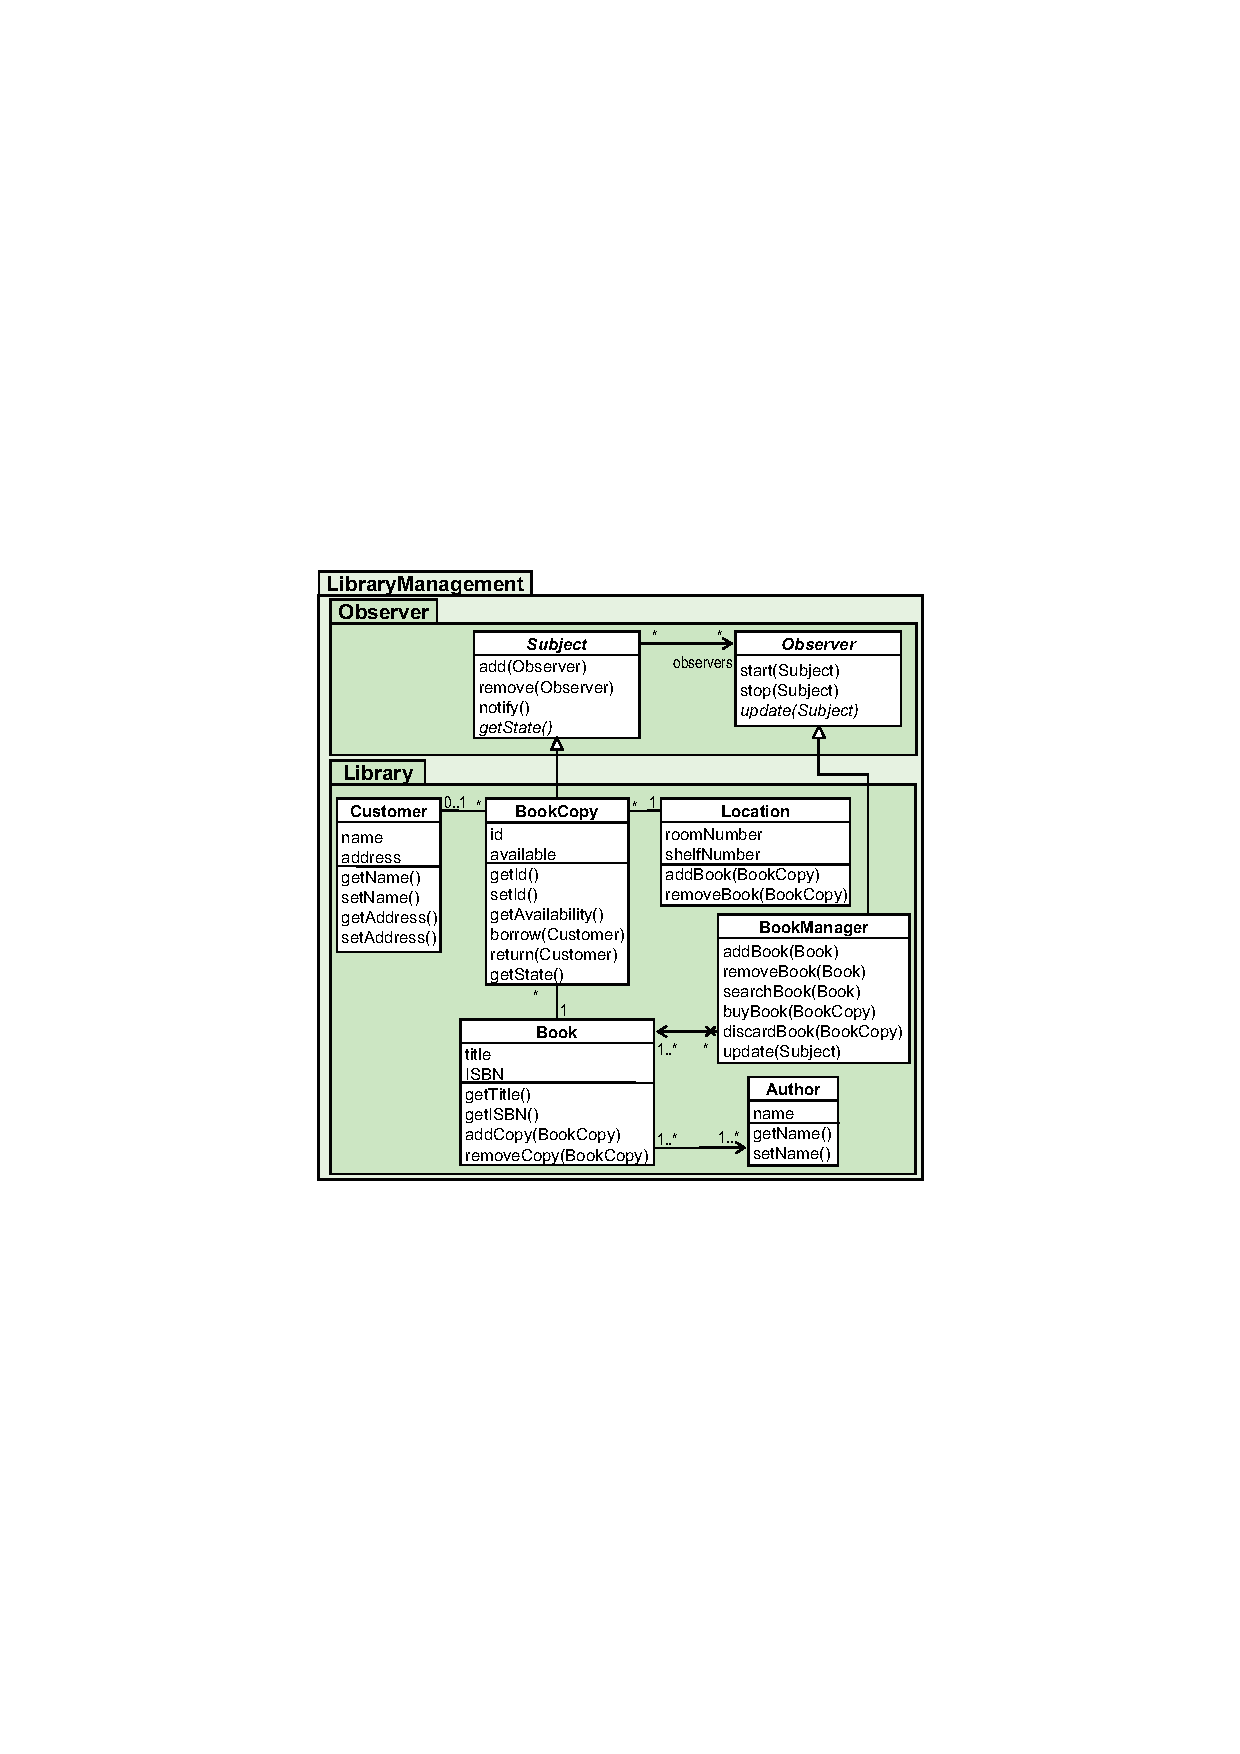
\includegraphics[width=0.7\textwidth]{chapters/figures/figure1}
	\caption{Sample figure}
	\label{fig:samplefigure_pdf}
\end{figure}


\section{Fonts}

When introducing important terms for the first time use \emph{emphasize}. For a consistent look and feel of proper names like {\cd} and {\uml{Observer}} pattern you may define macros in the main document \texttt{thesis.tex}.

\section{Code}

For short code fragments use the \textit{verbatim} environment.

\begin{verbatim}
//Start Program
System.out.println("Hello World!");
//End Program
\end{verbatim}

A much better alternative is the \textit{algorithm} environment (cf. Algorithm~\ref{alg:samplealgorithm}). This environment offers special formatting features for loops, operations and comments.

\begin{algorithm}[h!]
\SetKwData{Left}{left}
\SetKwData{This}{this}
\SetKwData{Up}{up}
\SetKwFunction{Union}{Union}
\SetKwFunction{FindCompress}{FindCompress}
\SetKwInOut{Input}{input}
\SetKwInOut{Output}{output}

\Input{A bitmap $Im$ of size $w\times l$}
\Output{A partition of the bitmap}

\BlankLine

\emph{special treatment of the first line}\;
\For{$i\leftarrow 2$ \KwTo $l$}{
\emph{special treatment of the first element of line $i$}\;
\For{$j\leftarrow 2$ \KwTo $w$}{\label{forins}
\Left$\leftarrow$ \FindCompress{$Im[i,j-1]$}\;
\Up$\leftarrow$ \FindCompress{$Im[i-1,]$}\;
\This$\leftarrow$ \FindCompress{$Im[i,j]$}\;
\If(\tcp*[r]{O(\Left,\This)==1}){\Left compatible with \This}{\label{lt}
\lIf{\Left $<$ \This}{\Union{\Left,\This}}\;
\lElse{\Union{\This,\Left}\;}
}
\If(\tcp*[r]{O(\Up,\This)==1}){\Up compatible with \This}{\label{ut}
\lIf{\Up $<$ \This}{\Union{\Up,\This}}\;
\tcp{\This is put under \Up to keep tree as flat as possible}\label{cmt}
\lElse{\Union{\This,\Up}}\tcp*[r]{\This linked to \Up}\label{lelse}
}
}
\lForEach{element $e$ of the line $i$}{\FindCompress{p}}
}
\caption{Sample algorithm}\label{alg:samplealgorithm}
\end{algorithm}



%%%%%%%%%%%%%%%%%%%%%%%%%%%%%%%%%%%%%%%%%
\chapter{Bibliographic Issues}
\label{ch:bibliographic}
%%%%%%%%%%%%%%%%%%%%%%%%%%%%%%%%%%%%%%%%%

%\section{Literature Search}
%
%Information on online libraries and literature search, e.g., interesting magazines, journals, conferences, and organizations may be found at \url{http://www.big.tuwien.ac.at/teaching/info.html}.
%
%\section{BibTeX}
%
%BibTeX should be used for referencing.
%
%The \LaTeX source document of this pdf document provides you with different samples for references to journals~\cite{jour:B2BServices}, conference papers~\cite{proc:TheWebMLApproachi}, books~\cite{book:umlatwork}, book chapters~\cite{incoll:ErhardKonrad1992}, electronic standards~\cite{man:BPEL}, dissertations~\cite{phdthesis:manuelWimmer}, masters' theses~\cite{mast:AUMLProfile}, and web sites~\cite{misc:BIGWebsite}. The respective BibTeX entries may be found in the file \texttt{references.bib}. For administration of the BibTeX references we recommend \url{http://www.citeulike.org} or JabRef for offline administration, respectively.
bruckner-2006-EVV\cite{proc:bruckner-2006-EVV}\\
ruiz \cite{proc:ruiz-2008-SEV} \\
Li:2008\cite{proc:Li:2008:AGI} \\
og/AgrawalaPHHKHT\cite{journals/tog/AgrawalaPHHKHT03}\\
roc:conf/si3d/NiederauerHAH03\cite{proc:conf/si3d/NiederauerHAH03}\\
Viola-05-Smart\cite{Viola-05-Smart}\\
journals/cacm/MitraYYLA13\cite{journals/cacm/MitraYYLA13}\\
Ward:2010:IDV:1893097\cite{Ward:2010:IDV:1893097}\\


%%%%%%%%%%%%%%%%%%%%%%%%%%%%%%%%%%%%%%%%%
%%% BACKMATTER %%%%%%%%%%%%%%%%%%%%%%%%%%
%%%%%%%%%%%%%%%%%%%%%%%%%%%%%%%%%%%%%%%%%
\appendix

\bibliographystyle{plain}
\bibliography{chapters/references}

\end{document}